%%%%%%%%%%%%%%%%% DO NOT CHANGE HERE %%%%%%%%%%%%%%%%%%%% 
%%%%%%%%%%%%%%%%%%%%%%%%%%%%%%%%%%%%%%%%%%%%%%%%%%%%%%%%%%{
    \documentclass[twoside,11pt]{article}
    %%%%% PACKAGES %%%%%%
    \usepackage{pgm2016}
    \usepackage{amsmath}
%    \usepackage{algorithm}
%    \usepackage[noend]{algpseudocode}
    \usepackage{subcaption}
    \usepackage[english]{babel}	
    \usepackage{paralist}	
    \usepackage[lowtilde]{url}
    \usepackage{fixltx2e}
    \usepackage{listings}
    \usepackage{color}
    \usepackage{hyperref}
    
    \usepackage{auto-pst-pdf}
    \usepackage{pst-all}
    \usepackage{pstricks-add}
    
    %%%%% MACROS %%%%%%
    \algrenewcommand\Return{\State \algorithmicreturn{} }
    \algnewcommand{\LineComment}[1]{\State \(\triangleright\) #1}
    \renewcommand{\thesubfigure}{\roman{subfigure}}
    \definecolor{codegreen}{rgb}{0,0.6,0}
    \definecolor{codegray}{rgb}{0.5,0.5,0.5}
    \definecolor{codepurple}{rgb}{0.58,0,0.82}
    \definecolor{backcolour}{rgb}{0.95,0.95,0.92}
    \lstdefinestyle{mystyle}{
       backgroundcolor=\color{backcolour},  
       commentstyle=\color{codegreen},
       keywordstyle=\color{magenta},
       numberstyle=\tiny\color{codegray},
       stringstyle=\color{codepurple},
       basicstyle=\footnotesize,
       breakatwhitespace=false,        
       breaklines=true,                
       captionpos=b,                    
       keepspaces=true,                
       numbers=left,                    
       numbersep=5pt,                  
       showspaces=false,                
       showstringspaces=false,
       showtabs=false,                  
       tabsize=2
    }
    \lstset{style=mystyle}
%%%%%%%%%%%%%%%%%%%%%%%%%%%%%%%%%%%%%%%%%%%%%%%%%%%%%%%%%% 
%%%%%%%%%%%%%%%%%%%%%%%%%%%%%%%%%%%%%%%%%%%%%%%%%%%%%%%%%% }

%%%%%%%%%%%%%%%%%%%%%%%% CHANGE HERE %%%%%%%%%%%%%%%%%%%% 
%%%%%%%%%%%%%%%%%%%%%%%%%%%%%%%%%%%%%%%%%%%%%%%%%%%%%%%%%% {
\newcommand\course{CS 330-001}
\newcommand\courseName{Introduction to Operating Systems}
\newcommand\semester{Winter 2020}
\newcommand\assignmentNumber{1}                             % <-- ASSIGNMENT #
\newcommand\studentName{Your Name}                  % <-- YOUR NAME
\newcommand\studentEmail{email@uregina.ca}          % <-- YOUR NAME
\newcommand\studentNumber{200XXYYZZ}                % <-- STUDENT ID #
%%%%%%%%%%%%%%%%%%%%%%%%%%%%%%%%%%%%%%%%%%%%%%%%%%%%%%%%%% }
%%%%%%%%%%%%%%%%%%%%%%%%%%%%%%%%%%%%%%%%%%%%%%%%%%%%%%%%%%

%%%%%%%%%%%%%%%%% DO NOT CHANGE HERE %%%%%%%%%%%%%%%%%%%% 
%%%%%%%%%%%%%%%%%%%%%%%%%%%%%%%%%%%%%%%%%%%%%%%%%%%%%%%%%%
%{

    \ShortHeadings{University of Regina -  \course ~~ \courseName}{\studentName - \studentNumber}
    \firstpageno{1}
    
    \begin{document}
    
    \title{Assignment \assignmentNumber}
    
    \author{\name \studentName \email \studentEmail \\
    \studentNumber
    \addr
    }
    
    \maketitle
%%%%%%%%%%%%%%%%%%%%%%%%%%%%%%%%%%%%%%%%%%%%%%%%%%%%%%%%%%
%%%%%%%%%%%%%%%%%%%%%%%%%%%%%%%%%%%%%%%%%%%%%%%%%%%%%%%%%% }

This is an example of how to cite:
\cite{darwiche00} proposed a new approach for inference in Bayesian networks (BNs) \citep{pear88}  based on partial differentiation called \emph{Arithmetic Circuits} \citep{darwiche00}.

This template is organized as follows.
In Section \ref{sec:background}, $\ldots$


\section{Example Section}
\label{sec:background}

%%EXAMPLE EQUATION

A \emph{joint probability distribution} (JPD) is function $P$ on the Cartesian product $V$ of the variable domains such that the following two conditions hold: 
\begin{align}
	&0 \leq P(v) \leq 1.0\text{ for each configuration $v \in V$; and}\\ \label{eq_01}		
	&\sum_{v \in V}{P(v)} = 1.0
\end{align}

Referring to Equation \ref{eq_01} here.

%EXAMPLE MULTIPLE TABLES TABLE

\begin{table}[!htb]

    \caption{Table (a) provides the prior probability of variable $A$ and Table (b) provides the conditional probability of $B$ given $A$.}
    \begin{subtable}{.5\linewidth}
      \centering
        \caption{}
        \begin{tabular}{c|c}
            $A$ & $P(A)$ \\ \hline
            1 & 0.3 \\
            0 & 0.7
        \end{tabular}
        \label{sub_table}
    \end{subtable}%
    \begin{subtable}{.5\linewidth}
      \centering
        \caption{}
        \begin{tabular}{cc|c}
            $A$ & $B$ & $P(B|A)$ \\ \hline
            1 & 1 & 0.1 \\
            1 & 0 & 0.9 \\
            0 & 1 & 0.8 \\
            0 & 0 & 0.2 \\
        \end{tabular}
    \end{subtable} 
        \label{subtb:pa}
\end{table}

Referring to Table \ref{subtb:pa} (\subref{sub_table}) here.

\subsection{Example Subsection}

%%EXAMPLE MATH INLINE
This is how you use math items inline: 
($\theta_a \star \lambda_a$), 
($\theta_{ab} \star \lambda_{{b}}$), 
($\theta_{a{\bar b}} \star \lambda_{{\bar b}}$),
($\lambda_{{b}} \star \theta_{{\bar a}b}$),
($\lambda_{{\bar b}} \star \theta_{{\bar a}\bar{b}}$), and
($\lambda_{{\bar a}} \star \theta_{{\bar a}}$).


Referring to Figure \ref{fig:deri}. 



\newpage %goes to a new page

%% EXAMPLE ALGORITHM
\begin{lstlisting}[language=python]
import numpy as np
from keras.models import Sequential
from keras.layers.core import Dense, Dropout, Layer, Activation
import time
import tensorflow as tf

f = open("results.csv", "w")


INPUT_SIZE = 10
OUTPUT_SIZE = INPUT_SIZE
nb_class = 3

batch_size = 128
nb_epoch = 40

np.random.seed(123)

X_train = np.random.rand(INPUT_SIZE, nb_class)
Y_train = np.random.rand(OUTPUT_SIZE, nb_class)

X_test = np.random.rand(INPUT_SIZE)
Y_test = np.random.rand(OUTPUT_SIZE)

for i in range(1,51):

    start_time = time.time()

    model = Sequential()
    model.add(Dense(INPUT_SIZE, input_shape=(nb_class,)))
    model.add(Activation('linear'))
    model.add(Dense(OUTPUT_SIZE))
    model.add(Activation('linear'))
    model.compile(loss='categorical_crossentropy', optimizer='rmsprop')

    final_time = time.time()
    diff_time = final_time - start_time

    f.write(str(i)+","+str(diff_time)+","+"\n")

f.close() 
\end{lstlisting}
 

\begin{table}[!h]
	\begin{center}
	\caption{Comparison of parallel and serial solutions for ACs with 50 runs each}
%	  \resizebox{\columnwidth}{!}{
	  \begin{tabular}{ l | cc }
Solution & Time average & Standard deviation \\ \hline
Serial		& 	0.1610		&	0.0536	\\
Parallel 	& 	0.0434		&	0.0082
		\label{tab:bench_bns}
	\end{tabular}
%	}
  	\end{center}
\end{table}

\begin{figure}[H]
    \begin{center}
    	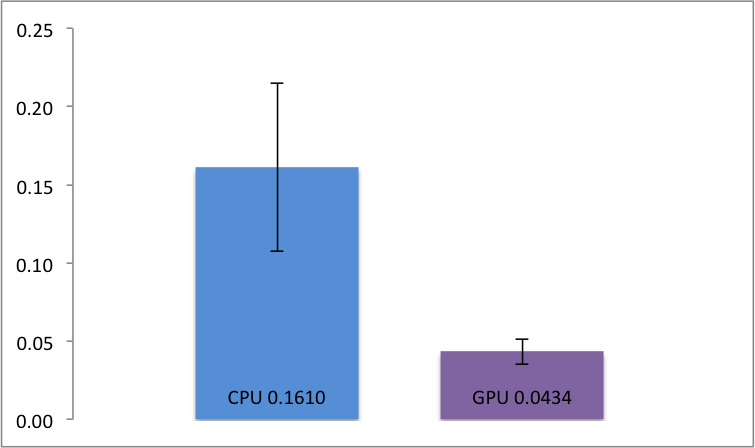
\includegraphics[width=0.7\columnwidth]{figures/graph.png}
		\caption{Comparison between CPU and GPU implementation of AC compiling.}
		\label{fig:deri}
    \end{center}
\end{figure}

\section{Conclusion}
\label{sec:conc}

In nec hendrerit arcu. Pellentesque leo libero, fringilla consectetur sapien eget, placerat finibus justo. Aliquam id sapien in eros lacinia euismod. Sed consectetur eros quis dui vestibulum pulvinar. Suspendisse ligula lacus, blandit interdum convallis sit amet, vulputate eget quam. Curabitur justo nunc, efficitur vitae fringilla eget, suscipit vitae sem. Etiam ultricies, nibh dictum convallis viverra, ipsum magna vehicula nibh, eu elementum purus est ac risus. Suspendisse sollicitudin auctor urna vel aliquet. In at eros et elit mollis lacinia. Fusce auctor leo id metus porttitor, vulputate semper erat congue. Donec rutrum erat non mauris convallis, id feugiat velit facilisis. Sed interdum magna sit amet mauris elementum pellentesque.

%% HERE IS WHERE THE REFERENCES IS INCLUDED
%% TO ADD NEW ONES, GO TO THE FILE references.bib IN THE REFERENCES FOLDER AND ADD IN bibtex FORMAT
\vskip 0.2in
\bibliography{references/references} 



\end{document}
